% Chapter 3 - Method
\section{Method}\label{chap:chap_3}

The methodology chapter outlines the approaches and tools used in this bachelor thesis. The primary objective of the study is to leverage the criticality in RL with the use of Deep Q-Networks (DQN) to obtain effective TL in conjunction with \emph{Highway-Env} and \emph{Merge-Env} environments. For development and implementation purposes of the RL agent, which will be capable of navigating and interacting with the given environment, the \texttt{Stable-Baselines3} framework was used. The visualisation was realised by the use of \texttt{matplotlib} and \texttt{seaborn} libraries.

\begin{figure}[H]
    \centering
    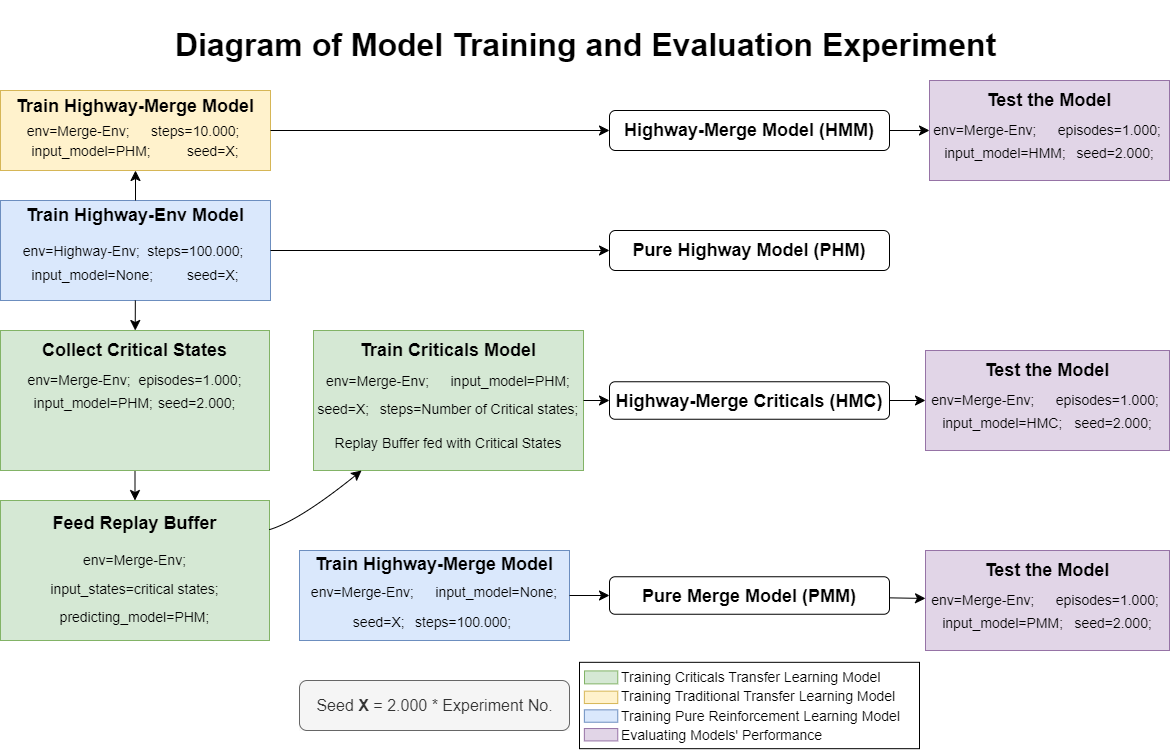
\includegraphics[width=\textwidth]{images/Diagram.png}
    \caption{The diagram, representing the progress of every experiment including preparation, training and evaluation steps.}
    \label{fig:diagram}
\end{figure}

\subsection{Environments: Highway-Env and Merge-Env}\label{sec:environments}

The operation of the RL agents in this thesis is realised within two environments: \emph{Highway-Env}~\cite{highway-env} and \emph{Merge-Env}. Those are realistic yet controlled simulations of autonomous driving tasks, that provide a setting for evaluating RL algorithms in various driving scenarios. Both environments model traffic behaviour, including surrounding vehicles and multiple lanes, allowing the agent to navigate dynamically and interact with nearby traffic. The environment provides rewards depending on the RL agent's behaviour on a highway; the agent has to avoid crashes while optimizing speed and deciding about proper lane positioning.

The \emph{Highway-Env} simulation environment is widely used for research in autonomous driving. Simulating a multi-lane highway encourages the agent vehicle to navigate in traffic, perform collision avoidance, and behave efficiently throughout driving. The following features are included in the environment:

\begin{itemize}
    \item \textbf{Dynamic Traffic:} Realistic behaviour of neighbouring traffic, simulating lane changing behaviour and velocity adjustments;

    \item \textbf{Reward Structure:} Actions that maintain safe and efficient driving are rewarded, while dangerous and unsafe situations are penalized. The agent can receive a reward for the correct choice of lane, avoiding collisions and retaining a higher speed;

    \item \textbf{Observation:} One perceives the surrounding world through observations of the velocities, positions, and relative distances of surrounding cars.
\end{itemize}

\begin{figure}[H]
    \centering
    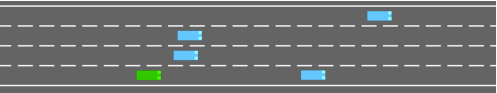
\includegraphics[width=\textwidth]{images/Highway.png}
    \caption{\emph{Highway-Env} render.}
    \label{fig:iterations_plot}
\end{figure}

To perform the TL and to challenge the agent in handling mode complex situations, the second environment was introduced -- \emph{Merge-Env}. This is a modified version of \emph{Highway-Env}, which specializes in merging scenarios. In \emph{Merge-Env} agent is targeted to navigate in merging situations, maintaining a smooth join of vehicles from on-ramps into main highway traffic. Performing timely decisions, velocity control and judging traffic gaps is what the agent desired to do in this environment to ensure effective, safe and smooth merging. Following additional complexity is added to this environment:

Merging Dynamics: On-ramp vehicles, that are trying to fuse into the highway, create an unpredictable traffic nature, forcing the agent to adapt quickly;
Challenging Scenarios: Merging raises the complexity level of decision-making, as safety and efficiency have to be maintained while coordinating its actions with merging traffic;
Enhanced Observations: Observations additionally include the velocity, position and relative distances of merging lane vehicles.

\begin{figure}[H]
    \centering
    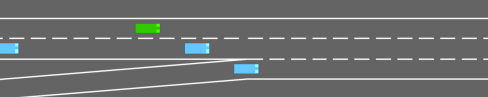
\includegraphics[width=\textwidth]{images/Merge.png}
    \caption{\emph{Merge-Env} render.}
    \label{fig:iterations_plot}
\end{figure}

Gymnasium API~\cite{towers2024gymnasiumstandardinterfacereinforcement} is a standardised RL interface used for the implementation of both environments. It has a modular and flexible framework which allows compatibility with popular RL libraries, such as StableBaselines3. Thus, the seamless integration of ready-to-use algorithms is enabled, allowing high training and evaluation efficiency in the chosen environments.

A combination of two environments creates a testbed for the performance evaluation of RL agents, as for autonomous driving scenarios. By a combination of those environments, this thesis aims to assess the effectiveness of TL concerning handling complex tasks, which contributes to the improvement of safety and efficiency in autonomous driving.

\subsubsection{Action Space}\label{sec:action_space}

Action Space defines possible actions to be considered in training, decision-making and evaluating processes. The \emph{Highway-Env} and \emph{Merge-Env} are implementations where the action space can be chosen to be either Discrete, Continuous, or Discrete Meta-Actions. The continuous action space in these environments means mainly that the velocity and steering angle of the agent can take arbitrary values in a predefined range. By controlling velocity and steering angle values, lane change, braking, overtaking, and other actions can be realized throughout the simulated traffic. However, the variety of actions makes the training and decision-making process more complex as the agent can leave the borders of the simulated highway. 

The discrete action space is a quantized continuous space, which is represented as a uniformly distributed grid of possible values for throttle and steering angle. Despite the size of the action space being gradually decreased compared to the continuous space, there is a third, simplest controlling action space to be used for this thesis: the Discrete Meta-Actions space. 

The Discrete Meta-Action space consists of 5 predefined actions which can replace the continuous action space. These actions are a tolerable replacement of continuous and discrete actions, which make the action space smaller and cover the most demanding actions of the agent. The available actions are~\cite{highwayenv2025}:

\begin{itemize}
    \item \texttt{IDLE} -- the velocity and steering angle are not adapted compared to the previous state;
    \item \texttt{LANE\_LEFT} -- the velocity value is saved unchanged, while the agent steers the vehicle to the left, changing the lane completely. In case the agent occupies the far-left lane, this action is not included in the possible action space; if the action is taken despite being unavailable, the \texttt{IDLE} action is performed;
    \item \texttt{LANE\_RIGHT} -- the velocity value is saved unchanged, while the agent steers the vehicle to the right, changing the lane completely. In case the agent occupies the far-right lane, this action is not included in the possible action space; if the action is taken despite being unavailable, the \texttt{IDLE} action is performed;
    \item \texttt{FASTER} -- the steering angle remains unchanged, while velocity is increased;
    \item \texttt{SLOWER} -- the steering angle remains unchanged, while velocity is decreased.
\end{itemize}

\subsection{Stable-Baselines3}

The \texttt{Stable-Baselines3} is a library that includes some of the most popular, efficient and reliable RL algorithms, that can be easily applied and used for different environment types like \emph{Highway-Env} and \emph{Merge-Env}. The list of implemented algorithms consists of Proximal Policy Optimization (PPO), Soft-Actor-Critic (SAC), and the algorithm that was used in this paper, Deep Q-Network (DQN). The privilege of the \texttt{Stable-Baselines3} is the simplicity of the Application Programming Interface (API), built on top of PyTorch, providing the ease of use of implemented models, requiring only a few lines of code to initialise, train and utilise the RL, which will be able to control the agent based on the learned policy~\cite{stable-baselines3}. Moreover, the developed API is not a black-box structure, but has open code, clear user guides and a huge number of active users that published struggles and solutions online, which was crucial during the implication of criticality throughout this thesis paper.

\subsection{Deep Q-Network (DQN)}\label{sec:dqn}

The RL algorithm used is Deep Q-Network (DQN). This algorithm combines the properties of "reinforcement learning with a class of artificial neural networks"~\cite{mnih2015human}. Following the combination of different RL approaches makes it possible for the DQN to handle environments with large state spaces, where the autonomous driving task is one example of such. The interaction with the environment is the main source of experience for the agent to learn an optimal policy. This algorithm was originally developed by Mnih et al.~\cite{mnih2015human}, where they introduced it as a method to address the RL challenges with high-dimensional state spaces through the use of deep learning, especially to estimate the Q-function throughout the learning process.

The core idea behind DQN is the process of the approximation of the Q-function based on the outputs of the deep neural network, giving an estimated reward based on the given current state and the action performed by the agent in this state. This algorithm performs self-education based on the gained experience and tries to maximize the cumulative rewards by making decisions and optimizing its actions. The Bellman equation is the one used to compute the value for state-action pair recursively through expected furture rewards:

\begin{equation}
    Q(s, a) = \mathbb{E} \left[ r + \gamma \max_{a'} Q(s', a') \mid s, a \right]
    \label{eq:bellman}
\end{equation}

where:
\begin{itemize}
    \item $Q(s, a)$ is the optimal action-value function,
    \item $r$ is the immediate reward received after taking action $a$ in state $s$,
    \item $\gamma \in [0,1]$ is the discount factor, controlling the importance of future rewards,
    \item $s'$ is the next state,
    \item $a'$ is the action taken in the next state,
    \item The expectation $\mathbb{E}$ represents averaging over possible next states and rewards.
\end{itemize}

The Q-values update is realised by Bellman equation with the help of deep neural network. The loss fulction used by DQN referes to TD error $\mathcal{L}(\theta)$:

\begin{equation}
    \mathcal{L}(\theta) = \mathbb{E} \left[ \left( y_t - Q(s, a; \theta) \right)^2 \right]
    \label{eq:dqn_loss}
\end{equation}
    
where the target value $y_t$ is computed as:
    
\begin{equation}
    y_t = r + \gamma \max_{a'} Q(s', a'; \theta^-)
    \label{eq:dqn_target}
\end{equation}
    
Here, $\theta$ represents current Q-network parameters, and $\theta^-$ corresponds to periodically updated target network. The periodical update tends to stabilize the training. The approximation of optimal Q-values is improved by the iterative minimisation of the loss function. This results into better decision-making process over time.

Additionally, there is a feature introduced with the DQN---the Replay Buffer, which played a crucial role in the implementation of the criticality in my thesis. The Replay Buffer offers the opportunity to store past experiences in the following form: firstly, the observations of the current state are saved; then the action that was taken by the policy based on the observation of the state; and finally, rewards that were obtained as a result of the action taken in the current state, followed by the observations of the resultant state. With the use of this feature, the experience can be not only saved but also replayed. This innovation assists during the process of approximation of the Q-values, mitigating the issues of overestimation of those, and helping agents to maintain effective and efficient learning in complex environments.

In this study, the DQN algorithm was used to train the agent in \emph{Highway-Env}~\cite{highway-env} and \emph{Merge-Env} environments for it to be able to navigate the highway autonomously, maximizing rewards and minimizing penalties, for example, due to collisions. To optimize the training process and to reach better performance, some parameters of the DQN policy were tuned. For instance, hyperparameters, including the learning rate and exploration rate. The exploration rate shows the fraction of the actions where the exploration epsilon-greedy policy will be applied~\cite{tokic2011adaptive}. This means if the exploration rate is $p$ (taking the values from 0 to 1), during $100 \cdot p$ per cent of the training steps ($N$), the following behaviour of decision-making will occur: in step 1, actions will be taken randomly in 100\% of steps; further, up until step $N \cdot p$, the proportion of actions taken randomly, not depending on the learned policy, will decrease proportionally, and at the point of step $N \cdot p$ it will reach 0\%. The efficacy of exploration (random actions) compared to exploitation (following the learned policy) is extremely high at the beginning of the training, where the policy does not act effectively, and exploration helps in gaining various experiences.

The learning rate is another key hyperparameter that determines the training performance of a Deep Q-learning (DQN) model. It defines how much the model parameters are changed during the update after each training step. In the DQN algorithm, the learning rate controls the magnitude of adjustments of the neural network weight, based on gradient descent. During training, the weight update is performed according to the following rule:

\begin{equation}
    \theta \leftarrow \theta - \alpha \nabla_\theta \mathcal{L}(\theta)
    \label{eq:weights}
\end{equation}

where:
\begin{itemize}
    \item $\alpha$ is the learning rate,
    \item $\mathcal{L}(\theta)$ is the loss function (e.g., mean squared error).
\end{itemize}

Training becomes unstable if the learning rate is too high ($\alpha$ is large) because the model weights change too much, which can lead to oscillations or divergence. If the learning rate is too low ($\alpha$ is small), the learning process becomes slow and the model can get stuck in local minima or take excessive time to reach an acceptable level of performance. In the context of the thesis, using a correct learning rate in the DQN algorithm allows the agent to effectively learn complex scenarios such as highway driving or merging manoeuvres, minimizing errors and providing high-quality results.

To train the model, the following mandatory programming steps should be completed:

\begin{enumerate}
    \item \textbf{Initialise the environment:} Use the \emph{Highway-Env} or \emph{Merge-Env} for training purposes with the \texttt{gymnasium.make()} function from the Gymnasium library~\cite{towers2024gymnasiumstandardinterfacereinforcement}. 
    The \texttt{make()} function takes as input the name of the environment: \texttt{"highway-v0"} for \emph{Highway-Env} and \texttt{"merge-v0"} for \emph{Merge-Env}. 
    To reduce training time, the faster variant \texttt{"highway-fast-v0"} is used, which is a modified version of the original implementation with degraded simulation accuracy for better performance~\cite{highway-env}.

    \item \textbf{Initialise the learning model:} Create the learning model to be used for training and assign it to the variable \texttt{model}. 
    This thesis is based on the Deep Q-Learning (DQN) policy, implemented using the StableBaselines3 library~\cite{stable-baselines3}. 
    The \texttt{DQN()} policy class has multiple adjustable parameters, but only three are considered relevant for this setup:
    \begin{itemize}
        \item \textbf{Type of DQN policy:} Three options are available -- \texttt{"MlpPolicy"}, \texttt{"CnnPolicy"}, and \texttt{"MultiInputPolicy"}. 
        Use \texttt{"CnnPolicy"} for image inputs, \texttt{"MultiInputPolicy"} for dictionary inputs, and \texttt{"MlpPolicy"} (used here) for simple observations.
        \item \textbf{Environment:} Use the previously initialised environment.
        \item \textbf{Seed value:} Ensures reproducibility. Using the same seed value results in identical randomization sets.
    \end{itemize}

    \item \textbf{Start the training process:} Use the \texttt{model.learn()} function of the DQN class to begin training. 
    This function requires the number of training steps as input. 
    To track progress, use the \texttt{progress\_bar} argument and set it to \texttt{True} to display the training progress.

    \item \textbf{Save the trained model:} Use the \texttt{model.save()} function to save the trained model to a file. 
    This allows the model to be saved once and later loaded with \texttt{model.load()} for further use, such as visualization or continued training (e.g., TL).
\end{enumerate}


\subsection{Transfer Learning}\label{sec:transfer_learning}

The base model for knowledge transfer was trained on the \emph{Highway-Env}. While training the model, the agent was taught to:
\begin{itemize}
    \item Maintain a safe distance from the vehicle in front,
    \item Assess the possibility of performing a lane change,
    \item Execute lane change maneuvers,
    \item Accelerate or decelerate to manoeuvre in traffic and receive corresponding rewards,
    \item Behave in traffic to maximize rewards under particular conditions.
\end{itemize}

The obtained model had "experience" on the highway but none in merge scenarios. Despite this, the model could make decisions based on previous knowledge, handle operations in pre- and post-merge scenarios at a good level, and avoid collisions during merging, whether by chance or through learned behaviour. 

The target was, however, to obtain a policy that would operate the agent inside \emph{Merge-Env} efficiently enough for the policy to be called safe. This could have been achieved via direct learning, following the same path as with the highway. While this approach would not require additional implementations, it would be as expensive and time-consuming as training the first model. Since this thesis uses environments that roughly simulate real-life scenarios, the scale of research into RL allowed experiments like training the model purely on \emph{Merge-Env} for comparison purposes. In real-life cases, however, such experiments are impossible on a larger scale, which highlights the effectiveness of TL.

One approach is to use the pre-trained model for straightforward but less intensive learning. Instead of starting with an empty policy, the policy trained for the highway task is used as the initial policy state for the training process in merging. Because RL recursively uses the policy's experience and knowledge, inputting the trained model into the DQN accelerates the model’s learning process. Therefore, the second model was trained on \emph{Merge-Env} using 10 times fewer steps than the initial highway model. This resulted in a model to be validated in future work.

Reducing the number of steps due to the "experienced" input model provides cost and time advantages. However, the training data used during DQN learning is still random. The approach explored throughout this thesis is to organize the training data more effectively. For this purpose, criticality principles will be used.

\subsection{Criticality}\label{sec:criticality}

The decision-making process is highly power-consuming for people because different actions taken in a particular situation could lead to drastically diverging results. An identical principle is to be considered for the decision-making performed by the machine. Exceptional meaning to wrongly taken actions should be taken into account during autonomous driving. Decisions taken by the autonomous vehicle are in the end to be brought to real road scenarios, where the lives of drivers, passengers and other traffic participants are of exceptional value. Thus, special attention is to be paid to possible dangerous situations that might occur in various driving scenarios. 

Unfortunately, it is impossible to create a list of all potential situations that can be considered to be unsafe. However, there is one approach that can help the machine to identify if the state is dangerous, more precisely if any of the available actions in the given state can lead to a critical situation. The states where one or some of the possible actions lead to such situations are to be called critical state~\cite{criticality2019}.

\begin{figure}[H]
    \centering
    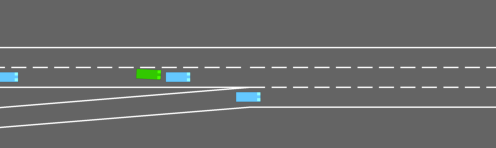
\includegraphics[width=\textwidth]{images/Critical_state.png}
    \caption{The state of a \emph{Merge-Env}, which was identified as critical.}
    \label{fig:iterations_plot}
\end{figure}

Figure \ref{fig:iterations_plot} demonstrates the state that was identified as critical. According to the position of the agent vehicle (green), the safest action among all available, described in Section \ref{sec:action_space}, will be \texttt{SLOWER}. The current velocity of the vehicle is unknown, therefore, the most meaningful action to take is decreasing velocity. Due to that one action favouring the decision-making, the value of criticality rose and the state was saved to be further used for leveraging criticality in TL.

The crucial role in decision-making is played by action values (Q-values). For a given state of the environment, each of the possible actions has its Q-value that was calculated by accumulating the possible prospected reward to be received if the action is taken. The calculations are performed according to the following formula~\cite{xue2023dvqn}:

\begin{equation}
Q^\pi(s, a) = \mathbb{E}_\pi \left[ \sum_{k=0}^\infty \gamma^k R_{t+k+1} \mid S_t = s, A_t = a, \pi \right]
\label{eq:q_value}
\end{equation}

where:
\begin{itemize}
    \item \( Q_\pi(s, a) \) is the action-value function, which represents the expected cumulative reward when starting in state \( s \), taking action \( a \), and following policy \( \pi \).
    \item \( \mathbb{E}_\pi [\cdot] \) denotes the expectation over all possible future trajectories, assuming actions are chosen according to policy \( \pi \).
    \item \( \sum_{k=0}^\infty \gamma^k R_{t+k+1} \) is the discounted sum of future rewards.
    \item \( \gamma \in [0,1] \) is the discount factor, which determines the importance of future rewards.
    \item \( R_{t+k+1} \) is the reward received at time step \( t+k+1 \).
    \item \( S_t \) is the state at time step \( t \).
    \item \( A_t \) is the action taken at time step \( t \).
    \item \( \pi \) represents the policy used to select actions.
\end{itemize}

In DQN the approximation of the action-value for every action is performed by the neural network. Then the policy performs the action which has the highest Q-value, according to:
\begin{equation}
 Q^*(s, a) = \max_\pi Q^\pi(s, a)
    \label{eq:max_q_value}
\end{equation}

To leverage the criticality in TL there was a complex procedure performed. The base model, trained purely on the \emph{Highway-Env}, was applied to perform "test drives" in the \emph{Merge-Env} to collect necessary data for the future applications of TL. The most important data to be collected for criticality purposes was: observations of all the completed steps throughout episodes. The model can give the Q-net of the observation out, which represents the Q-values for each of the 5 possible actions(described in Section 3.1.1). Based on the maximum action-value among those in Q-net, as described earlier, the algorithm was making decisions about which action to perform for a given observation. However, to find critical states the variance of Q-values was taken into account(calculated via \ref{eq:variance}).

The purpose of calculating the variance is to find the deviation of values inside of a Q-net, mainly to identify if one of the action values was reasonably higher than all others. Higher variance represents that one of the actions was much more likely to be taken by the policy than others. The Q-net variances of all the observations recorded should have been further analysed. Obtained values were analysed to find and save every local maximum throughout episodes. Finding the local maxima can be realised in multiple ways, for example via the derivative value of a function, however, the simpler method is to compare two neighbouring values. This algorithm was implemented into the scipy.signal.find\_peaks() function. 

Scipy library~\cite{Virtanen_2020} is an implementation of various scientific approaches with Python programming language. The subpackage \texttt{signal} focuses on various signal processing techniques and linear systems theory with a huge functionality including peak finding. The scipy.signal.find\_peaks() function does the following: it traverses the input 1D array while comparing the current value with two neighbouring values one from the right and one from the left, in case the value is greater than both neighbours, the value represents a local peak, otherwise, an algorithm continues. As an output, the function returns an array of peaks. To identify the observation that produced the following peak, the array of observations was traversed in parallel.

When observations of critical states are collected, the next goal is to use them for TL of the initial Highway policy. The ordinary DQN policy is trained in the way, that when the desired number of training epochs the algorithm uses the initial states of the system. Those are fed into the algorithm, and based on them the policy is trained. It either explores or exploits the initial state and the following states triggered by the action taken by the existing policy. Based on this experience the agent is trained to perform the decision-making in favour of one action in every given state, thus maximising rewards and, by that, the driving performance. However, the crucial point of initial state sampling for the training is that this is done randomly. Meaning every initial state of the system is randomly generated: the lane of the agent, the positions of surrounding vehicles, its velocities and the velocity of the agent car, everything is initialised randomly in every step.

The theory of this bachelor paper is, instead of a set of randomised states, to feed the DQN algorithm with a set of critical states of a smaller length and evaluate if an acceptable performance can be achieved via this method. The set of input states is generated by the DQN internally. This is performed by the Replay Buffer.

\subsection{Replay Buffer}\label{sec:replay_buffer}

As critical states are collected, the next processing step is feeding this set into the algorithm for purposes of TL. The target is to control the input of the DQN by replacing random state samples with a list of critical states. This was realised with the use of an in-built component of DQN called Replay Buffer(or Experience Replay).

The whole idea behind the principle of experience replay is grounded in neuroscience. Observing and exploring rodents, scientists suggest that the brain replays sequences of prior experience during its sleeping and awake resting phases~\cite{Foster2006}. Based on this knowledge DQN was extended by the Replay Buffer, where the design is following: experience, completed once will not be erased after one step, but on the contrary will be stored inside of the Replay Buffer to be reapplied later~\cite{schaul2016prioritizedexperiencereplay}. Moreover, it becomes more probable for the rare-appearing experience samples to be learned multiple times. Utilising a mix of recent and older experience stabilises the training process.

Google DeepMind's "Prioritized Experience Replay" ~\cite{schaul2016prioritizedexperiencereplay} research towards the optimisation of the usage of Replay Buffer in the DQN served as an inspiration for implementation within this thesis. The paper explores one possible improvement of a general Replay Buffer realisation, where the DQN will utilise the set of random states in a manner, where some states will be prioritized over others. The purpose of the research is brilliantly described in one sentence: "This paper addresses only the latter: making the most effective use of the replay memory for learning, assuming that its contents are outside of our control." After digging into the prioritised replay approach, the concept of overwriting the Replay Buffer data came to mind. Generally, the intention, that was pursued during the development of the Replay Buffer, was to reduce the amount of experience required for effective learning.

A list of observations is not all information, which is required to create a working buffer. Additionally, actions taken under the conditions of the state, the received reward and the resultant observations are required. To obtain the following data, the pre-trained highway model was used, which is the same model that collected critical states. Before the start of the transfer model training process, the experience buffer is filled with all necessary values and connected to a system to be employed by the DQN algorithm.
